\chapter{Introduzione}

Il riconoscimento dell'attività umana (Human Activity Recognition, HAR) è un campo molto attivo della ricerca e una
quantità sempre maggiore di tecniche di \textit{deep learning} sviluppate negli ultimi anni ha dimostrato di essere 
affidabile per la classificazione delle attività di vita quotidiana (Activities of Daily Living, ADLs).

Un aspetto che lega la quasi totalità delle tecniche messe in campo quando si parla di HAR è sicuramente l'ottenimento delle informazioni 
utili per le analisi. 

Esistono diverse tecniche di acquisizione usate per il riconoscimento delle attività. 
Tra le più utilizzate troviamo quelle basate sull'analisi di frame video o immagini, e quelle 
che impiegano i dati inerziali ottenuti dai sensori di movimento \cite{har_survey}.

\vspace{5mm} %5mm vertical space

In questa trattazione ho scelto l'uso dei dati inerziali per il riconoscimento delle attività.
Gli smartphone e gli indossabili (ad esempio braccialetti ed orologi intelligenti) sono sempre più comuni e perciò costituiscono 
una fonte di informazioni potenzialmente infinita.


\section{Dati inerziali}
Le informazioni relative al movimento di un corpo nello spazio tridimensionale sono raccolte 
dai cosiddetti \textbf{sensori inerziali}, principalmente accelerometro e giroscopio.
\subsubsection{Accelerometro}
L'accelerometro è un sensore capace di misurare l'accelerazione gravitazionale su un oggetto.
Un tempo destinato ad usi scientifici e militari, è diventato di uso comune con l'avanzare della tecnologia.

La totalità degli smartphone e degli indossabili intelligenti sono oggi dotati di un \textit{accelerometro a 3 assi} in grado 
di misurare l'accelerazione applicata su ognuno dei 3 assi dello spazio. 
Da questo deriva la possibilità di conoscere l'orientamento del dispositivo e di conseguenza i movimenti.

\subsubsection{Giroscopio}
Il giroscopio è un sensore capace di ricavare l'orientamento dell'oggetto sulla base di alcune proprietà fisiche che lo contraddistinguono.

Una buona parte di smartphone ed indossabili intelligenti sono dotati anche di un \textit{giroscopio a 3 assi} che coopera 
con l'accelerometro nella raccolta di dati inerziali.

\section{Classificazione}
Il riconoscimento delle attività si basa sulla \textit{classificazione}, un problema statistico che ha l'obiettivo di ipotizzare 
quale tra un insieme di etichette meglio definisce un insieme di caratteristiche. 

La classificazione, in informatica, è un ramo dell'apprendimento supervisionato (\textit{supervised learning}),
ovvero una branca dell'apprendimento automatico (\textit{machine learning}) che punta ad insegnare ad un sistema informatico una regola generale
di calcolo su un certo dominio di dati in modo che successivamente possa applicare in autonomia le stesse leggi anche a dati futuri.

Definiamo quindi \textbf{classificatore} un algoritmo in grado di risolvere il problema della classificazione, ovvero di fornire in output 
l'etichetta che meglio identifica i dati ricevuti in input.
Nel caso in esame il classificatore dovrà ipotizzare un'attività ricevendo in input un set di dati inerziali 
raccolti dall'applicazione sviluppata.

\subsection{L'importanza dei dati}
Ipotizzando che la qualità dei dati sia ottima (o almeno sufficiente), l'aspetto di cui bisogna assolutamente tener conto quando 
si parla di apprendimento automatico è la quantità di dati che si è in grado di raccogliere. 
L'efficienza e l'efficacia di un classificatore, in generale, si basano interamente sui valori precedentemente appresi.

La necessità di un set di dati ampio per l'apprendimento è principalmente conseguenza del fatto che non viviamo in un mondo ideale: 
le attività svolte nella vita reale non sono perfettamente suddivisibili per essere facilmente classificate e inoltre, dato che diverse persone
potrebbero svolgere una uguale attività in modi differenti, non si ha nemmeno una corrispondenza biunivoca tra un insieme di dati e l'attività \cite{framework_long_term_data_har}.


\newpage
\section{Obiettivo e panoramica del progetto}
Lo scopo del progetto è quindi lo sviluppo di un classificatore di ADLs in grado di interagire con una applicazione
Android.

\begin{figure}[H]
    \centering
    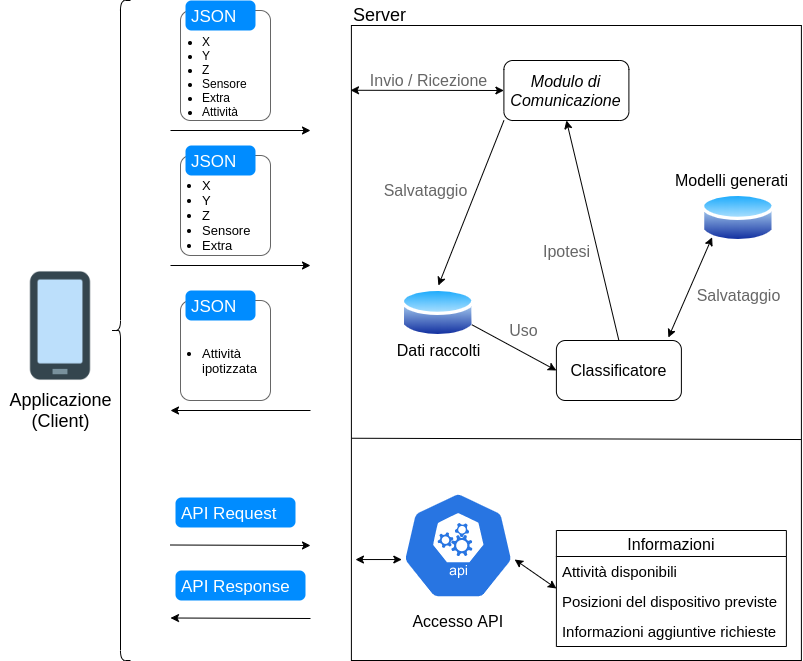
\includegraphics[scale = 0.50]{assets/images/overview.png}
    \caption{Panoramica del progetto}
    \label{fig:overview}
\end{figure}

\subsubsection{Applicazione}
L'applicazione permette, mediante l'utilizzo dei principali sensori inerziali del dispositivo, la raccolta dei dati che saranno poi elaborati 
remotamente. Si occupa inoltre di fornire all'utente un riscontro dell'attività ipotizzata in fase di analisi.
\subsubsection{RESTful Web API}
Useremo delle RESTful Web API personalizzate come fonte di informazioni iniziali.
\subsubsection{Messaggero}
Chiameremo \textit{messaggero} il componente server che si occupa dello scambio dati con il client. Tra i suoi compiti 
quello di immagazzinare i dati ricevuti e fornire le risposte.
\subsubsection{Classificatore}
Il classificatore gestisce la mole di valori ottenuta 
tentando di eseguire il riconoscimento vero e proprio delle attività 
per poi restituire l'ipotesi formulata.